\input{../include/preamble}

\title[ID1019 Dynamic programming]{Dynamic programming}
 

\author{Johan Montelius}
\institute{KTH}
\date{\semester}

\begin{document}

\begin{frame}
\titlepage
\end{frame}

\begin{frame}{Hinges and latches}

\pause Assume you're producing hinges and latches and would like to make as much money as possible.

\begin{columns}

 \begin{column}{0.4\linewidth}


\includegraphics[width=0.8\linewidth]{hinges.jpg}

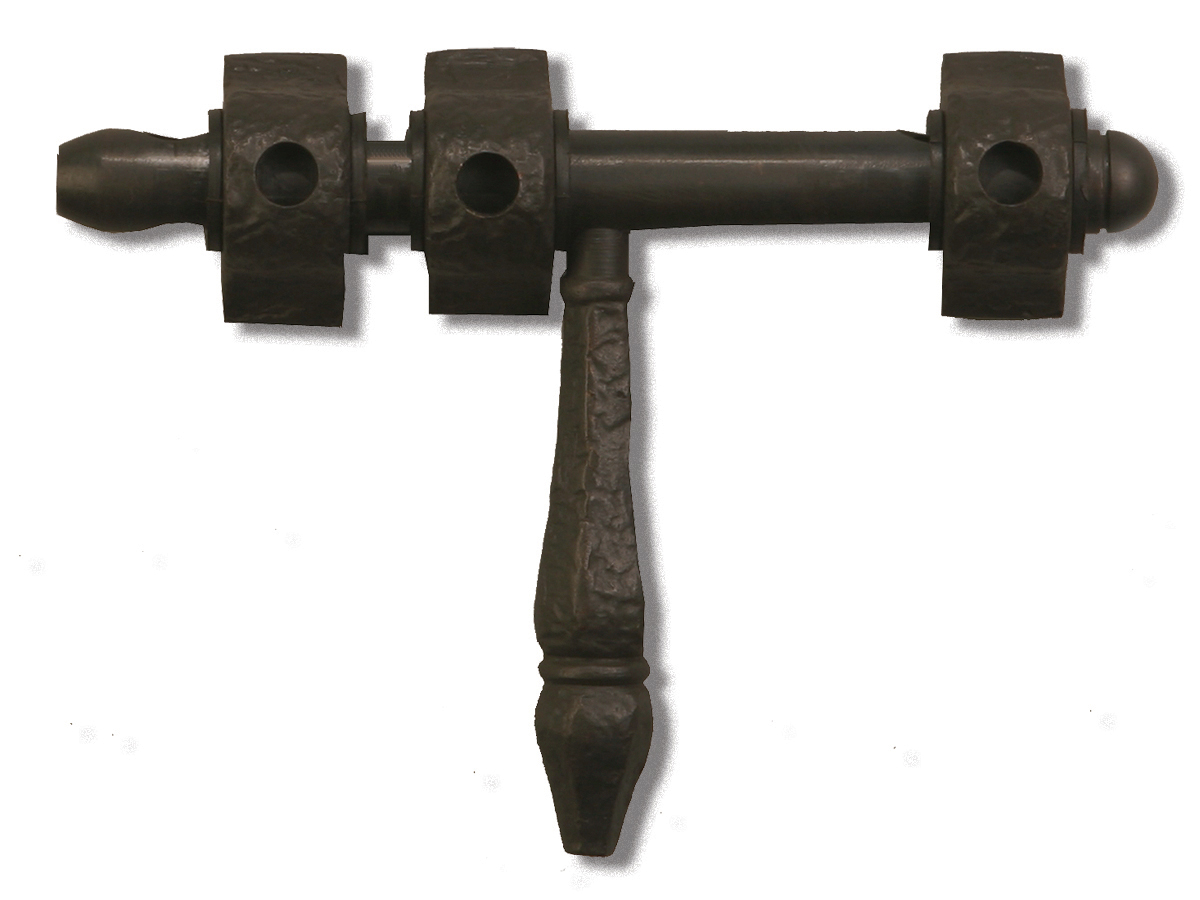
\includegraphics[width=0.8\linewidth]{latch.jpg}

 \end{column}
 \begin{column}{0.5\linewidth}
  \begin{itemize}
\pause\item Your resources are 2400g of raw material and 480 minutes of time.

\pause\item Each hinge takes 260g of material and 40 minutes to make.

\pause \item Each latch takes 180g of material and 60 minutes to make.

\pause \item Hinges are sold for 30 crowns and latches for 24 crowns.
  \end{itemize}
 \end{column}
\end{columns}
\pause \vspace{20pt}

How many hinges and latches should you produce to maximize profit. 

\end{frame}

\begin{frame}{Hinges and latches}

\pause Assume you're producing hinges and latches and would like to make as much money as possible.

\begin{columns}

 \begin{column}{0.4\linewidth}


\includegraphics[width=0.8\linewidth]{hinges.jpg}

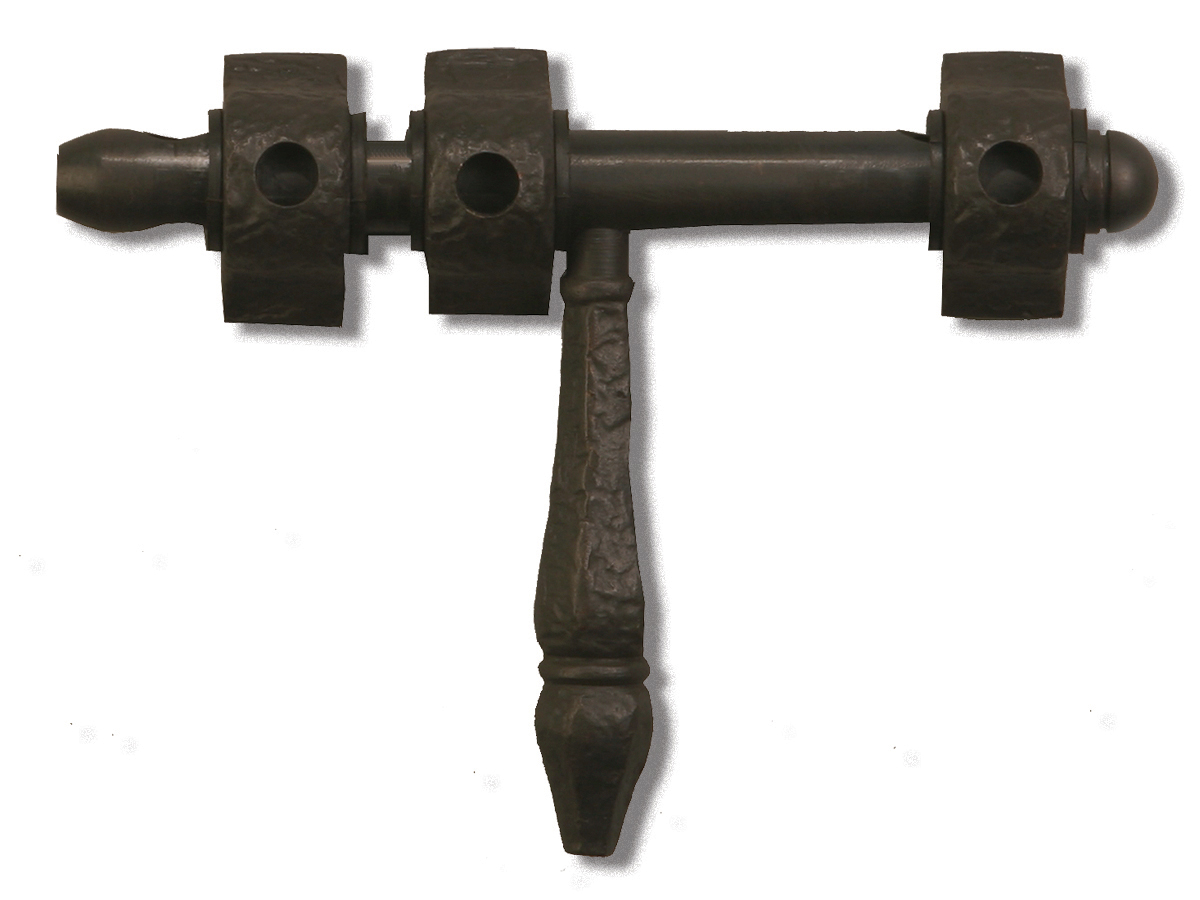
\includegraphics[width=0.8\linewidth]{latch.jpg}

 \end{column}
 \begin{column}{0.5\linewidth}
 Assume we make $h$ hinges and $l$ latches:
  \begin{itemize}
\pause\item limited resources: $260h + 180l < 2400$

\pause\item limited time: $40h + 60l < 480$

\pause \item profit: $p = 30h + 24l$

\pause \item find $h$ and $l$ to maximize $p$
  \end{itemize}
 \end{column}
\end{columns}
\pause \vspace{20pt}

How many hinges and latches should you produce to maximize profit. 

\end{frame}


\begin{frame}{linear programming}

\begin{columns}
 \begin{column}{0.5\linewidth}
\begin{figure}
\begin{tikzpicture}[
        scale=0.3,
        important line/.style={thick},
        axis/.style={very thick, ->, >=stealth'},
        dashed line/.style={dashed, thin},
        pile/.style={thick, ->, >=stealth', shorten >=2pt},
        every node/.style={color=black}
    ]

    % axis
    \draw[axis] (-1,0)  -- (16,0) node(xline)[right] {$hinges$};
    \draw[axis] (0,-1) -- (0,16) node(yline)[above] {$latches$};
    \pause
    \draw [dashed] (0,13.3) -- (9.2,0);
    \node [right] at (2,13) {$260h + 180l < 2400$};
    \pause
    \draw [dashed] (0,8) -- (12,0) {};
    %\draw [dashed] (0,10) -- (15,0) {};
    \node [right] at (14,4) {$40h + 60l < 480$};
\end{tikzpicture}
\end{figure}
 \end{column} 
 \begin{column}{0.5\linewidth}
  $$ p = 30h + 24l$$ 
  \pause
  maxium profit is found in one of the corners: \pause
  $$ h = 0, l = 8 \rightarrow  p = 192$$ \pause
  $$ h = 9, l = 0  \rightarrow  p = 270$$  \pause
  $$ h = 7, l = 3 \rightarrow p =  282$$ \pause
 \end{column}
 \end{columns}
\end{frame}

\begin{frame}{search for the answer}

To find the maximum profit, we either:

\pause \vspace{20pt}\hspace{40pt}
   make a hinge and then maximize profit or

\pause \vspace{20pt}\hspace{40pt}
   make a latch and then maximize profit.

\pause \vspace{20pt}\hspace{40pt}


\end{frame}


\begin{frame}[fragile]{search for the answer}

Describe a product as {\tt \{material, time, prize\}}: a hinge is {\tt \{260, 40, 30\}} and a latch is {\tt \{180, 60, 24\}}.

\pause\vspace{20pt}

Define a function {\tt search(material, time, hinge, latch)}, that
given an amount of material, time and descriptions of hinges and
latches, returns the number of hinges, $h$, and latches, $l$, to produce to
maximize profit $p$, {\tt \{h, l, p\}}.

\pause\vspace{20pt}

\begin{verbatim}
@spec seach(integer, integer, hinge, latch) :: {integer, integer, integer}

def search(material, time, hinge, latch) do 
   :
   :
  {hinges, latches, profit}
end
\end{verbatim}
\end{frame}


\begin{frame}[fragile]{search for the answer}

\begin{verbatim}
def search(m, t, {hm, ht, hp}=h, {lm, lt, lp}=l) when (m >= hm) and 
                                                      (t >= ht) and 
                                                      (m >= lm) and 
                                                      (t >= lt) ->
\end{verbatim}\pause
\begin{verbatim}
  ## we have material and time to make either a hinge or latch
  {hi, li, pi} = search((m-hm), (t-ht), h, l),
  {hj, lj, pj} = search((m-lm), (t-lt), h, l), 
\end{verbatim}\pause
\begin{verbatim}
  ## which alternative will give us the maximum profit
  if (pi+hp) > (pj+lp) do
    ## make hinge
    {(hi+1), li, (pi+hp)};
  else
    # make a latch
    {hj, (lj+1), (pj+lp)}
  end
end
\end{verbatim}
\end{frame}

\begin{frame}[fragile]{search for the answer}

\begin{verbatim}
   :
def search(m, t, {hm, ht, hp}=h, l) when (m >= hm) and (t >= ht)  do
  ## we can make a hinge
  {hn, ln, p} = search((m-hm), (t-ht), h, l)
  {hn+1, ln, (P+hp)}
end
\end{verbatim}\pause
\begin{verbatim}
def search(m, t, h, {lm, lt, lp}=l) when (m >= lm) and (t >= lt)  do
  ## we can make a latch
  {hn, ln, p} = search((m-lm), (t-lt), h, l)
  {hn, ln+1, p+lp}
end
\end{verbatim}\pause
\begin{verbatim}
def search(_, _, _, _) do
  ## we can make neither
  {0,0,0}
end
\end{verbatim}
\end{frame}


\begin{frame}[fragile]{a test}

\begin{verbatim}
>Hinges.search(2400, 480, {260, 40, 30}, {180, 60, 24}).
\end{verbatim}
\pause
\begin{verbatim}
{7, 3, 282}
\end{verbatim}
\pause
\begin{verbatim}
>Hinges.search(2000,480,{260,40,30},{180,60,24}).
\end{verbatim}
\pause
\begin{verbatim}
{4,5,240}
\end{verbatim}
\begin{verbatim}
>Hinges.search(2800,520,{260,40,30},{180,60,32}).
\end{verbatim}
\pause
\begin{verbatim}
{7,4,338}
\end{verbatim}

\end{frame}

\begin{frame}{problem solved}

\pause
\vspace{40pt}\hspace{140pt}What is the problem?

\end{frame}

\begin{frame}{complexity}

\begin{figure}
\begin{tikzpicture}[
        scale=0.5,
        important line/.style={thick},
        dashed line/.style={dashed, thin},
        every node/.style={color=black}
    ]
    \node [] at (14,20) {\texttt{search(2400,480, ...)}};
    \pause
    \draw [dashed] (14,19) -- (5,17);
    \node [] at (5,16) {\texttt{search(2140,440, ...)}};
    \pause
    \draw [dashed] (14,19) -- (21,17);
    \node [] at (21,16) {\texttt{search(2220,420, ...)}};
    \pause
    \draw [dashed] (5,15) -- (0,13);
    \node [] at (0,12) {\texttt{search(1880,400, ...)}};
    \pause
    \draw [dashed] (5,15) -- (10,13);
    \node [] at (10,12) {\texttt{search(2040,360, ...)}};
    \pause
    \draw [dashed] (0,11) -- (-2,9);    
    \draw [dashed] (0,11) -- (2,9);    
    \draw [dashed] (10,11) -- (8,9);    
    \draw [dashed] (10,11) -- (12,9);    
    \draw [dashed] (21,15) -- (19,13);    
    \draw [dashed] (21,15) -- (23,13);    
\end{tikzpicture}
\end{figure}

{\em What is the depth of this tree? How does it relate to the size of the resources?}
\end{frame}

\begin{frame}{complexity}

\begin{figure} 
 
\includegraphics[scale=0.5]{doomed.png}
\end{figure}


\end{frame}

\begin{frame}{the m x t space}

\begin{figure}
\begin{tikzpicture}[
        scale=0.6,
        important line/.style={thick},
        axis/.style={very thick, ->, >=stealth'},
        dashed line/.style={dashed, thin},
        pile/.style={thick, ->, >=stealth', shorten >=2pt},
        every node/.style={color=black}
    ]

    % axis
    \draw[axis] (-1,0)  -- (10,0) node(xline)[right] {material};
    \draw[axis] (0,-1) -- (0,10) node(yline)[above] {time};
    \pause
    \draw [pile, color=red] (0,0) -- +(2.6,2) node()[below right]{hinge}; 
    \pause
    \draw [pile, color=green] (0,0) -- +(1.8,3) node()[above left]{latch}; 
    % --------------------------------------
    \pause
    \draw [pile, color=red] (2.6,2) -- +(2.6,2); 
    \pause
    \draw [pile, color=green] (2.6,2) -- +(1.8,3); 
    \pause
    \draw [pile, color=red] (1.8,3) -- +(2.6,2) ; 
    \pause
    \draw [pile, color=green] (1.8,3) -- +(1.8,3); 
    % --------------------------------------

    \draw [pile, color=red] (5.2,4) -- +(2.6,2); 
    \draw [pile, color=green] (5.2,4) -- +(1.8,3); 
    \draw [pile, color=red] (4.4,5) -- +(2.6,2); 
    \draw [pile, color=green] (4.4,5) -- +(1.8,3); 
    \draw [pile, color=red] (3.6,6) -- +(2.6,2); 
    \draw [pile, color=green] (3.6,6) -- +(1.8,3); 


\end{tikzpicture}
\end{figure}
\end{frame}

\begin{frame}{dynamic programming}

\vspace{40pt}\hspace{100pt}\parbox[l][100pt][l]{200pt}{Problem divided into simpler parts that can be solved independently, but \pause

-  the parts share sub-problems that can be reused.}

\end{frame}


\begin{frame}[fragile]{Fibonacci}

\begin{columns}
 \begin{column}{0.5\linewidth}
\begin{verbatim}
def fib(0) do 0 end
def fib(1) do 1 end
def fib(n) do
    fib(n-1) + fib(n-2)
end
\end{verbatim}
 \end {column}
\pause
 \begin{column}{0.5\linewidth}
\begin{verbatim}
def fib(0) do {0, nil} end
\end{verbatim}
\pause
\begin{verbatim}
def fib(1) do {1, 0} end
\end{verbatim}
\pause
\begin{verbatim}
def fib(n) do
    {n1, n2} = fib(n-1) 
\end{verbatim}
\pause
\begin{verbatim}
    {n1+n2, n1}
end
\end{verbatim}
 \end {column}
\end{columns}

\end{frame}

\begin{frame}[fragile]{memory}

Let's add a memory to the search function. 

\begin{verbatim}
def memory(material, time, hinge, latch) do
  mem = Memory.new()
  {solution, _} = search(material, time, hinge, latch, mem)
  solution
end
\end{verbatim}\pause

\begin{verbatim}
def check(material, time, hinge, latch, mem) do
  case Memory.lookup({material,time}, mem) of
    nil ->
      ## no previous solution found
      {solution, mem} = search(material, time, hinge, latch, mem)
      {solution, Memory.store({material,time}, solution, mem)}
    found -> 
      {found, mem}
  end
end
\end{verbatim}

\end{frame}


\begin{frame}[fragile]{memory}

\begin{verbatim}
def search(m, t,..., mem) when ... do 
\end{verbatim}
\pause
\begin{verbatim}
    {..., mem} = check(...,  mem), 
\end{verbatim}
\pause
\begin{verbatim}
    {..., mem} = check(..., mem), 
\end{verbatim}
\pause
\begin{verbatim}
    if ...  do
      {..., mem};
\end{verbatim}
\pause
\begin{verbatim}
    else 
      {..., mem}
    end
  end
\end{verbatim}

\end{frame}

\begin{frame}[fragile]{a memory}

\vspace{10pt}\pause

the {\em key} is a tuple \texttt{\{m,t\}}, defining the remaining resource (the point in the mxt space).

\vspace{10pt}\pause

The {\em value} is the number of hinges and latches and best profit possible at this point \texttt{\{h, l, p\}}.

\vspace{10pt}\pause

The functions we should implement are: \pause

\begin{itemize}

  \item \texttt{new()}: returns a new memory \pause

  \item \texttt{store(k, v, mem)}: returns a new memory where the key
  \texttt{k} is associated with the value \texttt{v} \pause

  \item \texttt{lookup(k, mem)}: return the value \texttt{v} assocaued with
  the key or \texttt{nil} if not found
\end{itemize}

\end{frame}


\begin{frame}[fragile]{a key-value list}

Let's implement the memory as a list of tuples \texttt{\{k, v\}}.

\pause \vspace{10pt}
\begin{verbatim}
defmodule Memory do

def new() do [] end
\end{verbatim}

\pause\vspace{5pt}
\begin{verbatim}
def store(k, v, mem) do
\end{verbatim}
\pause
\begin{verbatim}
   [{k, v}|mem]
end
\end{verbatim}

\pause\vspace{5pt}
\begin{verbatim}
def lookup(_, []) do nil end
\end{verbatim}\pause
\begin{verbatim}
def lookup(k, [{k,v}|_]) do v end
\end{verbatim}
\pause
\begin{verbatim}
def lookup(k, [_|rest]) do lookup(k, rest) end
\end{verbatim}

\end{frame}

\begin{frame}{benchmark}

  {\em on a i7-4500 1.8GHz, time in ms}
  \vspace{10pt}

\hspace{100pt}\begin{tabular}{|c|c|c|c|c|}
\hline 
       m & t & m + t & search & memory \\
\hline
      1000&        200&       1200&         0.01&        0.03  \\
      2000&        400&       2400&         0.08&        0.08  \\
      3000&        600&       3600&         0.70&        0.13  \\
      4000&        800&       4800&           10&        0.35  \\
      5000&       1000&       6000& \pause   110& \pause 0.42 \\
      6000&       1200&       7200& \pause  1900& \pause 0.80 \\
      7000&       1400&       8400& \pause  32000& \pause 1.30 \\
      8000&       1600&       9600& \pause  550000& \pause 2.10 \\          
\hline
\end{tabular}

\end{frame}

\begin{frame}[fragile]{complexity}

\begin{columns}
\begin{column}{0.5\linewidth}
\begin{tikzpicture}[
        scale=0.5,
        important line/.style={thick},
        axis/.style={very thick, ->, >=stealth'},
        dashed line/.style={dashed, thin},
        pile/.style={thick, ->, >=stealth', shorten >=2pt},
        every node/.style={color=black}
    ]
    % axis
    \draw[axis] (-1,0)  -- (10,0) node(xline)[right] {material};
    \draw[axis] (0,-1) -- (0,10) node(yline)[above] {time};
    \draw [pile, color=red] (0,0) -- +(2.6,2);

    % --------------------------------------
    \draw [pile, color=red] (2.6,2) -- +(2.6,2); 
    \draw [pile, color=red] (5.2,4) -- +(2.6,2); 
    \draw [pile, color=green] (5.2,4) -- +(1.8,3);

\pause
    \draw [pile, color=green] (2.6,2) -- +(1.8,3); 
\pause
    \draw [pile, dashed, color=gray] (4.4,5) -- +(2.6,2);
\pause
    \draw [pile, color=green] (4.4,5) -- +(1.8,3);
\pause
    % --------------------------------------
\pause
    \draw [pile, color=green] (0,0) -- +(1.8,3);
\pause
    \draw [pile, dashed, color=gray] (1.8,3) -- +(2.6,2) ; 
\pause
    \draw [pile, color=green] (1.8,3) -- +(1.8,3); 
\pause
    \draw [pile, dashed, color=gray] (3.6,6) -- +(2.6,2); 
\pause
    \draw [pile, color=green] (3.6,6) -- +(1.8,3); 
\end{tikzpicture}

\end{column}
\begin{column}{0.5\linewidth}
\begin{verbatim}
def lookup(_, []) -> nil end
def lookup(k, [{k,v}|_]) do v end
def lookup(k, [_|rest]) do 
  lookup(k, rest)
end
\end{verbatim}

\end{column}
\end{columns}

\end{frame}

\begin{frame}[fragile]{a map}

Why not implement the memory as a hash map? 

\vspace{10pt}
\begin{verbatim}
defmodule Better do

def new() do %{} end
\end{verbatim}
\pause
\begin{verbatim}    
def store(k,v, mem) do 
  Map.put(mem, k, v)
end
\end{verbatim}
\pause
\begin{verbatim}        
def lookup(k, mem) do
  Map.get(mem, k)
end
\end{verbatim}

\end{frame}

\begin{frame}{benchmark}

  {\em on a i7-4500 1.8GHz, time in ms}
  \vspace{10pt}

\hspace{100pt}\begin{tabular}{|c|c|c|c|c|}
\hline 
       m & t & m+t & list & map\\
\hline
      1000&       200&      1200&      0.03&      0.06\\
      2000&       400&      2400&      0.11&      0.18\\
      3000&       600&      3600&      0.34&      0.24\\
      4000&       800&      4800&      0.82&      0.39\\
      5000&      1000&      6000&      1.26&      0.31\\
      6000&      1200&      7200&      1.53&      0.36\\
      7000&      1400&      8400&      2.25&      0.34\\
      8000&      1600&      9600&      2.94&      0.43\\
      9000&      1800&     10800&      4.22&      0.49\\
     10000&      2000&     12000&      6.22&      0.58\\
     11000&      2200&     13200&      8.97&      0.69\\
     12000&      2400&     14400&     12.55&      0.84\\
\hline
\end{tabular}


\end{frame}

\begin{frame}{benchmark}

\begin{figure}
 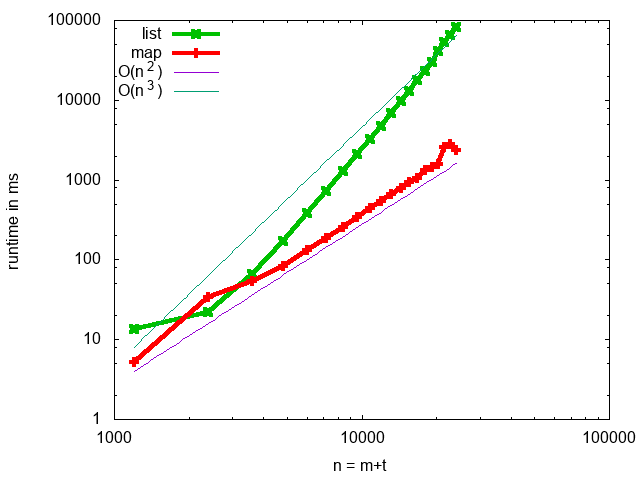
\includegraphics[scale=0.5]{map.png}
\end{figure}

\end{frame}

\begin{frame}{dynamic programming}

\vspace{40pt}\hspace{80pt}\parbox[l][60pt][l]{240pt}{Problem divided into simpler parts that can be solved independently, but 

\vspace{10pt}\pause
-  the parts share subproblems that can be reused and,

\vspace{10pt}\pause
-  we can memorize solutions of subproblems.
}



\end{frame}



\begin{frame}{shortest path}

Find the shortest path from one node to another.

\begin{figure}
\begin{tikzpicture}[scale=1,
        ->,>=stealth',shorten >=1pt,auto, node distance=80pt, semithick]

  \tikzstyle{every state}=[fill=red,draw=none,text=white]

  \node[initial,state] (A)                    {A};
  \node[state]         (B) [above right of=A] {B};
  \node[state]         (D) [below right of=A] {D};
  \node[state]         (C) [below right of=B] {C};
  \node[state]         (E) [above right of=C] {E};
  \node[state]         (F) [below right of=C] {F};
  \node[state]         (G) [below right of=E] {G};

  \path (A) edge              node {2} (B)
            edge              node {5} (D)
        (B) edge              node {2} (C)
            edge              node {3} (E)
        (C) edge              node {6} (E)
            edge              node {1} (G)
        (D) edge              node {3} (C)
            edge              node {2} (F)
        (E) edge              node {2} (G)
        (F) edge              node {3} (G)
            edge              node {1} (C);
\end{tikzpicture}
\end{figure}

{\em We assume the graph is a ``Directed Acyclic Graph'' (DAG)}

\end{frame}

\begin{frame}{dynamic programming aproach}

\begin{columns}
 \begin{column}{0.4\linewidth}
\begin{figure}
\begin{tikzpicture}[scale=0.6,
        ->,>=stealth',shorten >=1pt,auto, node distance=40pt, semithick]

  \tikzstyle{every state}=[fill=red,draw=none,text=white,minimum size=10pt]

  \node[initial,state] (A)                    {A};
  \node[state]         (B) [above right of=A] {B};
  \node[state]         (D) [below right of=A] {D};
  \node[state]         (C) [below right of=B] {C};
  \node[state]         (E) [above right of=C] {E};
  \node[state]         (F) [below right of=C] {F};
  \node[state]         (G) [below right of=E] {G};

  \path (A) edge              node {2} (B)
            edge              node {5} (D)
        (B) edge              node {2} (C)
            edge              node {3} (E)
        (C) edge              node {6} (E)
            edge              node {1} (G)
        (D) edge              node {3} (C)
            edge              node {2} (F)
        (E) edge              node {2} (G)
        (F) edge              node {3} (G)
            edge              node {1} (C);
\end{tikzpicture}
\end{figure}
 \end{column}
 \begin{column}{0.6\linewidth}
   The {\em dynamic programming approach}: 
   \begin{itemize}
     \item find a recursive solution
     \item memorize solutions to subproblems
   \end{itemize}
 \end{column}
\end{columns}

\end{frame}

\begin{frame}[fragile]{dynamic programming aproach}

\begin{columns}
 \begin{column}{0.4\linewidth}
  If we are in the final node the distance is zero and the path is \[\].

  \vspace{10pt}
  Otherwise, for each outgoing edge: find the shortest path from the
  reached node and return the shortest given the distance to the node.

 \end{column}
 \begin{column}{0.6\linewidth}
  \begin{verbatim}
def shortest(from, from, _) do  {0, []} end
  \end{verbatim}
  \pause
  \begin{verbatim}
def shortest(from, to, graph) do
  next = Graph.next(from, graph)
  distances = distances(next, to, graph)
  select(distances)
end
  \end{verbatim}
  \pause {\em If no path is found we should return {\tt \{:inf, nil\}}}.
 \end{column}
\end{columns}

\end{frame}

\begin{frame}[fragile]{a graph}

How do we represent a graph?

\begin{columns}
 \begin{column}{0.4\linewidth}
\begin{figure}
\begin{tikzpicture}[scale=0.6,
        ->,>=stealth',shorten >=1pt,auto, node distance=40pt, semithick]

  \tikzstyle{every state}=[fill=red,draw=none,text=white,minimum size=10pt]

  \node[initial,state] (A)                    {A};
  \node[state]         (B) [above right of=A] {B};
  \node[state]         (D) [below right of=A] {D};
  \node[state]         (C) [below right of=B] {C};
  \node[state]         (E) [above right of=C] {E};
  \node[state]         (F) [below right of=C] {F};
  \node[state]         (G) [below right of=E] {G};

  \path (A) edge              node {2} (B)
            edge              node {5} (D)
        (B) edge              node {2} (C)
            edge              node {3} (E)
        (C) edge              node {6} (E)
            edge              node {1} (G)
        (D) edge              node {3} (C)
            edge              node {2} (F)
        (E) edge              node {2} (G)
        (F) edge              node {3} (G)
            edge              node {1} (C);
\end{tikzpicture}
\end{figure}
 \end{column}
 \begin{column}{0.6\linewidth}
  As a list of edges: 

\texttt{[\{:a, :b, 2\}, \{:a, :d, 5\}, \{:b, :c, 2\} ... ]}

\pause \vspace{10pt}

  As a list of nodes:

\begin{verbatim}
[{:a, [{:b, 2}, {:d, 5}]}, 
 {:b, [{:c, 2}, {:e, 3}]}, 
 ...]
\end{verbatim}

\pause \vspace{10pt}

  As a matrix of edges:

\begin{verbatim}
{{ nil, 2 ,nil, 5 ,nil,nil,nil}, 
 { nil,nil, 2 ,nil, 3 ,nil,nil}, 
  ...}}
\end{verbatim}

\end{column}
\end{columns}

\end{frame}

\begin{frame}[fragile]{a graph}

How about this?

\begin{columns}
 \begin{column}{0.4\linewidth}
\begin{figure}
\begin{tikzpicture}[scale=0.6,
        ->,>=stealth',shorten >=1pt,auto, node distance=40pt, semithick]

  \tikzstyle{every state}=[fill=red,draw=none,text=white,minimum size=10pt]

  \node[initial,state] (A)                    {A};
  \node[state]         (B) [above right of=A] {B};
  \node[state]         (D) [below right of=A] {D};
  \node[state]         (C) [below right of=B] {C};
  \node[state]         (E) [above right of=C] {E};
  \node[state]         (F) [below right of=C] {F};
  \node[state]         (G) [below right of=E] {G};

  \path (A) edge              node {2} (B)
            edge              node {5} (D)
        (B) edge              node {2} (C)
            edge              node {3} (E)
        (C) edge              node {6} (E)
            edge              node {1} (G)
        (D) edge              node {3} (C)
            edge              node {2} (F)
        (E) edge              node {2} (G)
        (F) edge              node {3} (G)
            edge              node {1} (C);
\end{tikzpicture}
\end{figure}
 \end{column}
 \begin{column}{0.6\linewidth}
\begin{verbatim}
 g = {:g, []}
 e = {:e, [{g , 2}]}
 c = {:c, [{g, 1}, {e, 6}]}
 f = {:f, [{c, 1}, {g, 3}]}
 d = {:d, [{f, 2}, {c, 3}]}
 b = {:b, [{c, 2}, {e, 3}]}
 a = {:a, [{b, 2}, {d, 5}]}
 
 [a: a, b: b, c: c, d: d, e: e, f: f, g: g]
 \end{verbatim}
\pause
{\em What has this to do with topological order?}
\end{column}
\end{columns}

\end{frame}


\begin{frame}[fragile]{the graph}

  Assume we represent a graph by a map indxed by nodes. Each node holds a key-value list of edges.

\begin{verbatim}
defmodule Graph do 

  def sample() do
    new([a: [b: 2, d: 5], b: [c: 2], ... ])
  end
\end{verbatim}
  
\begin{verbatim}
  def new(nodes) do
    Map.new(nodes)
  end

  def next(from, map) 
    Map.get(map, from, [])
  end
end
\end{verbatim}

\end{frame}

\begin{frame}[fragile]{distances}

  Find the distance to the destination from each of the next steps.

\vspace{20pt} \pause
  
\begin{verbatim}
def distances(next, to, graph) do
\end{verbatim}
\pause
\begin{verbatim}
    Enum.map(next, fn({n,d}) ->   
\end{verbatim}
\pause
\begin{verbatim}
                   case shortest(n, to, graph) do
\end{verbatim}
\pause
\begin{verbatim}
                        {:inf, nil} -> {:inf, nil};
\end{verbatim}
\pause
\begin{verbatim}
                        {k, path} -> {d+k, [n|path]}
\end{verbatim}
\pause
\begin{verbatim}
                   end
                end)
end
\end{verbatim}
\end{frame}

\begin{frame}[fragile]{select}

Select the smallest path in the list: \texttt{[\{9, [:d, :c, :g]\}, ..]}

\vspace{10pt}\pause

\begin{verbatim}
  def select(distances) do
    List.foldl(distances,
      {:inf, nil},
      fn ({d,_}=s,{ad,_}=acc) ->
        if d < ad do
          s
        else
          acc
        end
      end)
  end
\end{verbatim}

\pause\vspace{10pt}{\em If the list is empty, the result could be {\tt \{:inf, nil\}}}.
\end{frame}

\begin{frame}[fragile]{dynamic programming aproach}

\begin{columns}
 \begin{column}{0.4\linewidth}
  If we are in the final node, the distance is zero and the path is \[\].

  \vspace{10pt}
  Otherwise, for each outgoing edge: find the shortest path from the
  reached node and return the shortest given the distance to the node.

 \end{column}
 \begin{column}{0.6\linewidth}
   \begin{verbatim}
def shortest(from, from, _) -> {0, []} end
  \end{verbatim}
  \pause
  \begin{verbatim}
def shortest(from, to, graph) do
  next = Graph.next(from, graph)
  distances = distances(next, to, graph)
  select(distances)
end
  \end{verbatim}
 \end{column}
\end{columns}

\pause\vspace{20pt}{\em What is the complexity?}

\end{frame}

\begin{frame}[fragile]{let's add a memory}

\begin{verbatim}
def dynamic(from, to, graph) do
  mem = Memory.new()
  {solution, _} = shortest(from, to, graph, mem)
  solution
end
\end{verbatim}

\pause\vspace{10pt}

{\em shortest(from, to, graph, mem) should return \{shortest path, updated memmory\}}

\pause\vspace{10pt}
\begin{verbatim}
def shortest(from, from, _, mem) do
    {{0, []}, ...}
end
def shortest(from, to, graph, mem) do
    next = Graph.next(from, graph),
    {..., ...} = distances(next, to, graph, mem)
    shortest = select(...)
    {..., ...}
end
\end{verbatim}

\end{frame}

\begin{frame}[fragile]{shortest path given memeory}

\pause\vspace{10pt}

{\em For all next steps, find the shortesta path.}

\pause\vspace{10pt}

\begin{verbatim}
  def distances(next, to, graph, mem) do
    List.foldl(next, {[], mem},
      fn ({t,d}, {dis,mem}=acc) ->
        case check(t, to, graph, mem) do
          {{:inf, _}, _} ->
            acc
          {{n, path}, mem} ->
            {[{d+n, [t|path]}| dis ], mem}
        end
      end)
  end
\end{verbatim}
\end{frame}

\begin{frame}[fragile]{shortest path given memeory}

{\em If a solution exists use it, if not - compute it.}

\begin{verbatim}
  def check(from, to, graph, mem) do
    case Memory.lookup(from, mem) do
      nil ->
        {solution, mem} = shortest(from, to, graph, mem)
        {solution,  Memory.store(from, solution, mem)}
     solution ->
        {solution, mem}
    end
  end
\end{verbatim}
\end{frame}



\begin{frame}{what if?}

\begin{figure}
\begin{tikzpicture}[scale=1,
        ->,>=stealth',shorten >=1pt,auto, node distance=80pt, semithick]

  \tikzstyle{every state}=[fill=red,draw=none,text=white]

  \node[initial,state] (A)                    {A};
  \node[state]         (B) [above right of=A] {B};
  \node[state]         (D) [below right of=A] {D};
  \node[state]         (C) [below right of=B] {C};
  \node[state]         (E) [above right of=C] {E};
  \node[state]         (F) [below right of=C] {F};
  \node[state]         (G) [below right of=E] {G};

  \path (A) edge              node {2} (B)
            edge              node {5} (D)
        (B) edge              node {2} (C)
            edge              node {3} (E)
        (C) edge              node {6} (E)
            edge              node {1} (G)
            edge              node {2} (A)        
        (D) edge              node {3} (C)
            edge              node {2} (F)
        (E) edge              node {2} (G)
        (F) edge              node {3} (G)
            edge              node {1} (C);
\end{tikzpicture}
\end{figure}

\end{frame}

\begin{frame}{Summary}


\vspace{40pt}\hspace{80pt}\parbox[l][60pt][l]{240pt}{Problem divided into simpler parts that can be solved independently, but 

\vspace{10pt}\pause
-  the parts share subproblems that can be reused and,

\vspace{10pt}\pause
-  we can memorize solutions of subproblems.
}

\end{frame}
\end{document}
